\documentclass{standalone}
\usepackage{tikz}
\usetikzlibrary{patterns, positioning}

\begin{document}
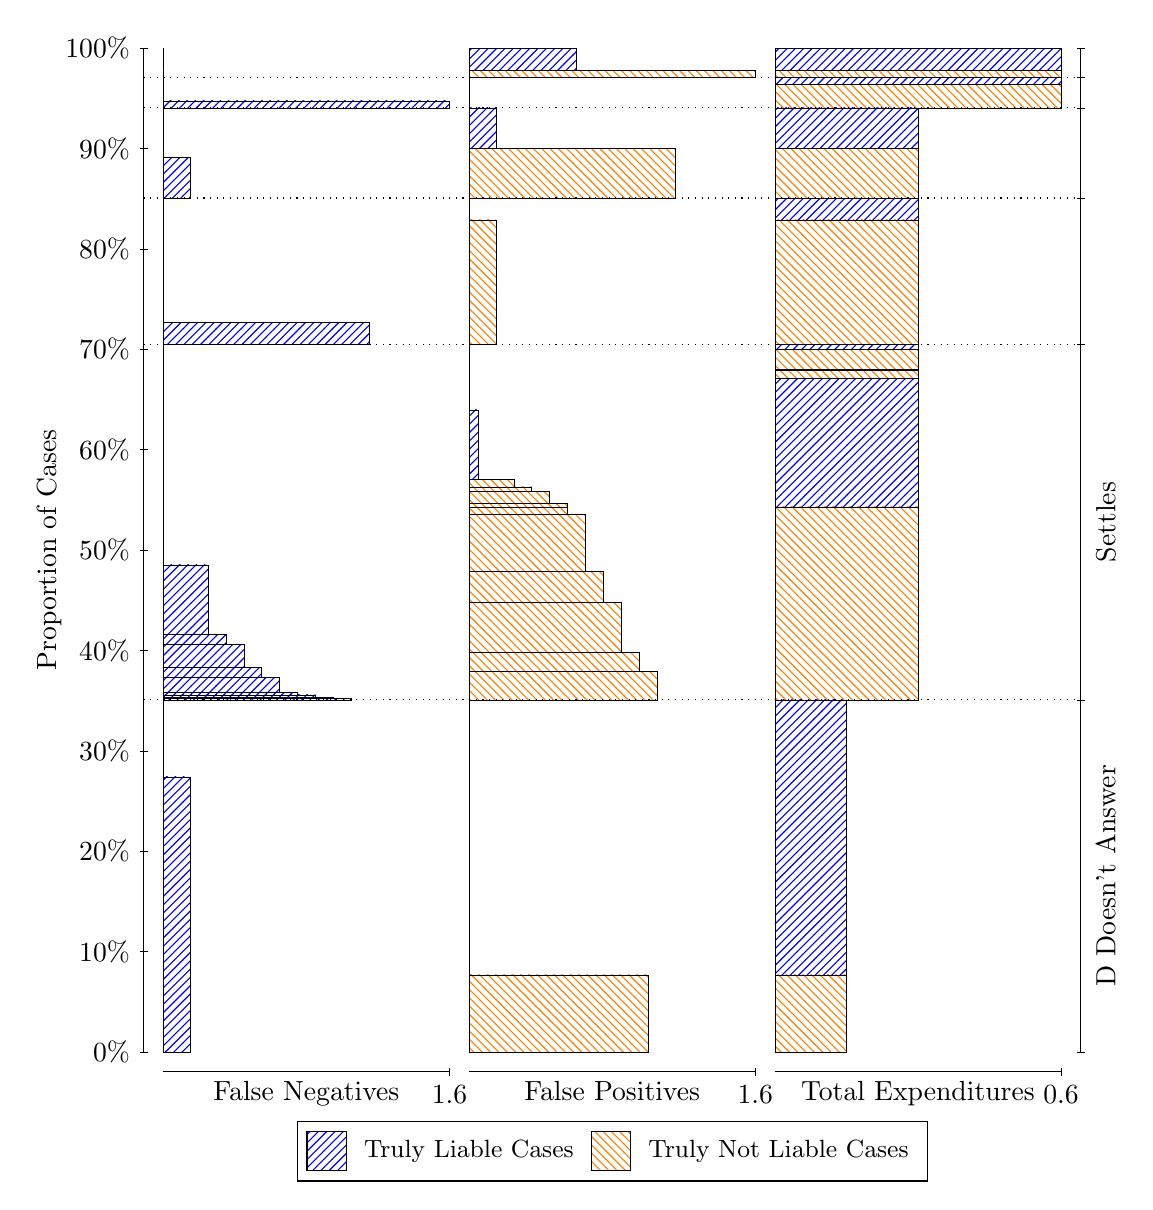
\begin{tikzpicture}
\draw[black, very thin] (1.5,1.75) -- (1.5,14.5);
\node[rotate=90, anchor=center] at (0.3, 8.125) {Proportion of Cases};
\draw[black, very thin] (1.45,1.75) -- (1.55,1.75);
\node[anchor=east] at (1.45, 1.75) {0\%};
\draw[black, very thin] (1.45,3.025) -- (1.55,3.025);
\node[anchor=east] at (1.45, 3.025) {10\%};
\draw[black, very thin] (1.45,4.3) -- (1.55,4.3);
\node[anchor=east] at (1.45, 4.3) {20\%};
\draw[black, very thin] (1.45,5.575) -- (1.55,5.575);
\node[anchor=east] at (1.45, 5.575) {30\%};
\draw[black, very thin] (1.45,6.85) -- (1.55,6.85);
\node[anchor=east] at (1.45, 6.85) {40\%};
\draw[black, very thin] (1.45,8.125) -- (1.55,8.125);
\node[anchor=east] at (1.45, 8.125) {50\%};
\draw[black, very thin] (1.45,9.4) -- (1.55,9.4);
\node[anchor=east] at (1.45, 9.4) {60\%};
\draw[black, very thin] (1.45,10.675) -- (1.55,10.675);
\node[anchor=east] at (1.45, 10.675) {70\%};
\draw[black, very thin] (1.45,11.95) -- (1.55,11.95);
\node[anchor=east] at (1.45, 11.95) {80\%};
\draw[black, very thin] (1.45,13.225) -- (1.55,13.225);
\node[anchor=east] at (1.45, 13.225) {90\%};
\draw[black, very thin] (1.45,14.5) -- (1.55,14.5);
\node[anchor=east] at (1.45, 14.5) {100\%};

\draw[black, very thin] (13.4,1.75) -- (13.4,14.5);
\draw[black, very thin] (13.35,1.75) -- (13.45,1.75);
\node[anchor=west] at (13.35, 1.75) {};
\draw[black, very thin] (13.35,6.222) -- (13.45,6.222);
\node[anchor=west] at (13.35, 6.222) {};
\draw[black, very thin] (13.35,10.738) -- (13.45,10.738);
\node[anchor=west] at (13.35, 10.738) {};
\draw[black, very thin] (13.35,12.595) -- (13.45,12.595);
\node[anchor=west] at (13.35, 12.595) {};
\draw[black, very thin] (13.35,13.741) -- (13.45,13.741);
\node[anchor=west] at (13.35, 13.741) {};
\draw[black, very thin] (13.35,14.129) -- (13.45,14.129);
\node[anchor=west] at (13.35, 14.129) {};
\draw[black, very thin] (13.35,14.5) -- (13.45,14.5);
\node[anchor=west] at (13.35, 14.5) {};

\draw[black, very thin, pattern color=blue, pattern=north east lines] (1.75,1.75) rectangle (2.0906,5.2443);
\draw[black, very thin, pattern color=orange, pattern=north west lines] (1.75,5.2443) rectangle (1.75,6.222);
\draw[black, very thin, pattern color=blue, pattern=north east lines] (1.75,6.222) rectangle (4.1344,6.2376);
\draw[black, very thin, pattern color=blue, pattern=north east lines] (1.75,6.2376) rectangle (3.9073,6.25);
\draw[black, very thin, pattern color=blue, pattern=north east lines] (1.75,6.25) rectangle (3.6802,6.284);
\draw[black, very thin, pattern color=blue, pattern=north east lines] (1.75,6.284) rectangle (3.4531,6.3203);
\draw[black, very thin, pattern color=blue, pattern=north east lines] (1.75,6.3203) rectangle (3.226,6.507);
\draw[black, very thin, pattern color=blue, pattern=north east lines] (1.75,6.507) rectangle (2.999,6.6337);
\draw[black, very thin, pattern color=blue, pattern=north east lines] (1.75,6.6337) rectangle (2.7719,6.9231);
\draw[black, very thin, pattern color=blue, pattern=north east lines] (1.75,6.9231) rectangle (2.5448,7.0554);
\draw[black, very thin, pattern color=blue, pattern=north east lines] (1.75,7.0554) rectangle (2.3177,7.936);
\draw[black, very thin, pattern color=orange, pattern=north west lines] (1.75,7.936) rectangle (1.75,10.738);
\draw[black, very thin, pattern color=blue, pattern=north east lines] (1.75,10.738) rectangle (4.3615,11.016);
\draw[black, very thin, pattern color=orange, pattern=north west lines] (1.75,11.016) rectangle (1.75,12.595);
\draw[black, very thin, pattern color=blue, pattern=north east lines] (1.75,12.595) rectangle (2.0906,13.112);
\draw[black, very thin, pattern color=orange, pattern=north west lines] (1.75,13.112) rectangle (1.75,13.741);
\draw[black, very thin, pattern color=blue, pattern=north east lines] (1.75,13.741) rectangle (5.3833,13.829);
\draw[black, very thin, pattern color=orange, pattern=north west lines] (1.75,13.829) rectangle (1.75,14.129);
\draw[black, very thin, pattern color=orange, pattern=north west lines] (1.75,14.129) rectangle (1.75,14.217);
\draw[black, very thin, pattern color=blue, pattern=north east lines] (1.75,14.217) rectangle (1.75,14.5);
\draw[black, very thin, pattern color=orange, pattern=north west lines] (5.6333,1.75) rectangle (7.9042,2.7277);
\draw[black, very thin, pattern color=blue, pattern=north east lines] (5.6333,2.7277) rectangle (5.6333,6.222);
\draw[black, very thin, pattern color=orange, pattern=north west lines] (5.6333,6.222) rectangle (8.0177,6.581);
\draw[black, very thin, pattern color=orange, pattern=north west lines] (5.6333,6.581) rectangle (7.7906,6.8238);
\draw[black, very thin, pattern color=orange, pattern=north west lines] (5.6333,6.8238) rectangle (7.5635,7.4627);
\draw[black, very thin, pattern color=orange, pattern=north west lines] (5.6333,7.4627) rectangle (7.3365,7.849);
\draw[black, very thin, pattern color=orange, pattern=north west lines] (5.6333,7.849) rectangle (7.1094,8.5725);
\draw[black, very thin, pattern color=orange, pattern=north west lines] (5.6333,8.5725) rectangle (6.8823,8.6715);
\draw[black, very thin, pattern color=orange, pattern=north west lines] (5.6333,8.6715) rectangle (6.8823,8.72);
\draw[black, very thin, pattern color=orange, pattern=north west lines] (5.6333,8.72) rectangle (6.6552,8.8723);
\draw[black, very thin, pattern color=orange, pattern=north west lines] (5.6333,8.8723) rectangle (6.4281,8.9276);
\draw[black, very thin, pattern color=orange, pattern=north west lines] (5.6333,8.9276) rectangle (6.201,9.0237);
\draw[black, very thin, pattern color=blue, pattern=north east lines] (5.6333,9.0237) rectangle (5.7469,9.9043);
\draw[black, very thin, pattern color=blue, pattern=north east lines] (5.6333,9.9043) rectangle (5.6333,10.738);
\draw[black, very thin, pattern color=orange, pattern=north west lines] (5.6333,10.738) rectangle (5.974,12.316);
\draw[black, very thin, pattern color=blue, pattern=north east lines] (5.6333,12.316) rectangle (5.6333,12.595);
\draw[black, very thin, pattern color=orange, pattern=north west lines] (5.6333,12.595) rectangle (8.2448,13.224);
\draw[black, very thin, pattern color=blue, pattern=north east lines] (5.6333,13.224) rectangle (5.974,13.741);
\draw[black, very thin, pattern color=orange, pattern=north west lines] (5.6333,13.741) rectangle (5.6333,14.042);
\draw[black, very thin, pattern color=blue, pattern=north east lines] (5.6333,14.042) rectangle (5.6333,14.129);
\draw[black, very thin, pattern color=orange, pattern=north west lines] (5.6333,14.129) rectangle (9.2667,14.217);
\draw[black, very thin, pattern color=blue, pattern=north east lines] (5.6333,14.217) rectangle (6.9958,14.5);
\draw[black, very thin, pattern color=orange, pattern=north west lines] (9.5167,1.75) rectangle (10.425,2.7277);
\draw[black, very thin, pattern color=blue, pattern=north east lines] (9.5167,2.7277) rectangle (10.425,6.222);
\draw[black, very thin, pattern color=orange, pattern=north west lines] (9.5167,6.222) rectangle (11.333,8.6715);
\draw[black, very thin, pattern color=blue, pattern=north east lines] (9.5167,8.6715) rectangle (11.333,10.309);
\draw[black, very thin, pattern color=orange, pattern=north west lines] (9.5167,10.309) rectangle (11.333,10.405);
\draw[black, very thin, pattern color=blue, pattern=north east lines] (9.5167,10.405) rectangle (11.333,10.421);
\draw[black, very thin, pattern color=orange, pattern=north west lines] (9.5167,10.421) rectangle (11.333,10.677);
\draw[black, very thin, pattern color=blue, pattern=north east lines] (9.5167,10.677) rectangle (11.333,10.738);
\draw[black, very thin, pattern color=orange, pattern=north west lines] (9.5167,10.738) rectangle (11.333,12.316);
\draw[black, very thin, pattern color=blue, pattern=north east lines] (9.5167,12.316) rectangle (11.333,12.595);
\draw[black, very thin, pattern color=orange, pattern=north west lines] (9.5167,12.595) rectangle (11.333,13.224);
\draw[black, very thin, pattern color=blue, pattern=north east lines] (9.5167,13.224) rectangle (11.333,13.741);
\draw[black, very thin, pattern color=orange, pattern=north west lines] (9.5167,13.741) rectangle (13.15,14.042);
\draw[black, very thin, pattern color=blue, pattern=north east lines] (9.5167,14.042) rectangle (13.15,14.129);
\draw[black, very thin, pattern color=orange, pattern=north west lines] (9.5167,14.129) rectangle (13.15,14.217);
\draw[black, very thin, pattern color=blue, pattern=north east lines] (9.5167,14.217) rectangle (13.15,14.5);
\draw[black, dotted] (1.5,6.222) -- (13.4,6.222);
\draw[black, dotted] (1.5,10.738) -- (13.4,10.738);
\draw[black, dotted] (1.5,12.595) -- (13.4,12.595);
\draw[black, dotted] (1.5,13.741) -- (13.4,13.741);
\draw[black, dotted] (1.5,14.129) -- (13.4,14.129);
\draw[black, very thin] (1.75,1.5) -- (5.3833,1.5);
\node[anchor=north] at (3.5667, 1.5) {False Negatives};
\draw[black, very thin] (5.3833,1.45) -- (5.3833,1.55);
\node[anchor=north] at (5.3833, 1.45) {1.6};

\draw[black, very thin] (5.6333,1.5) -- (9.2667,1.5);
\node[anchor=north] at (7.45, 1.5) {False Positives};
\draw[black, very thin] (9.2667,1.45) -- (9.2667,1.55);
\node[anchor=north] at (9.2667, 1.45) {1.6};

\draw[black, very thin] (9.5167,1.5) -- (13.15,1.5);
\node[anchor=north] at (11.333, 1.5) {Total Expenditures};
\draw[black, very thin] (13.15,1.45) -- (13.15,1.55);
\node[anchor=north] at (13.15, 1.45) {0.6};

\node[black, centered, rotate=90] at (13.72, 3.986) {D Doesn't Answer};
\node[black, centered, rotate=90] at (13.72, 8.4799) {Settles};





\draw (7.449999999999999,1.5) node[draw=none] (baseCoordinate) {};
\begin{scope}[align=center]
        \matrix[scale=0.5, draw=black, below=0.5cm of baseCoordinate, nodes={draw}, column sep=0.1cm]{
            \node[rectangle, draw, minimum width=0.5cm, minimum height=0.5cm, pattern=north east lines, pattern color=blue] {}; &
            \node[draw=none, font=\small] (B) {Truly Liable Cases}; &
            \node[rectangle, draw, minimum width=0.5cm, minimum height=0.5cm, pattern=north west lines, pattern color=orange] {}; &
            \node[draw=none, font=\small] (B) {Truly Not Liable Cases}; \\
            };
\end{scope}

\end{tikzpicture}
\end{document}